\documentclass{standalone}
\usepackage{tikz}
\usetikzlibrary{patterns, positioning}
\usepackage[sfdefault]{ClearSans} %% option 'sfdefault' activates Clear Sans as the default text font
\usepackage[T1]{fontenc}

\begin{document}
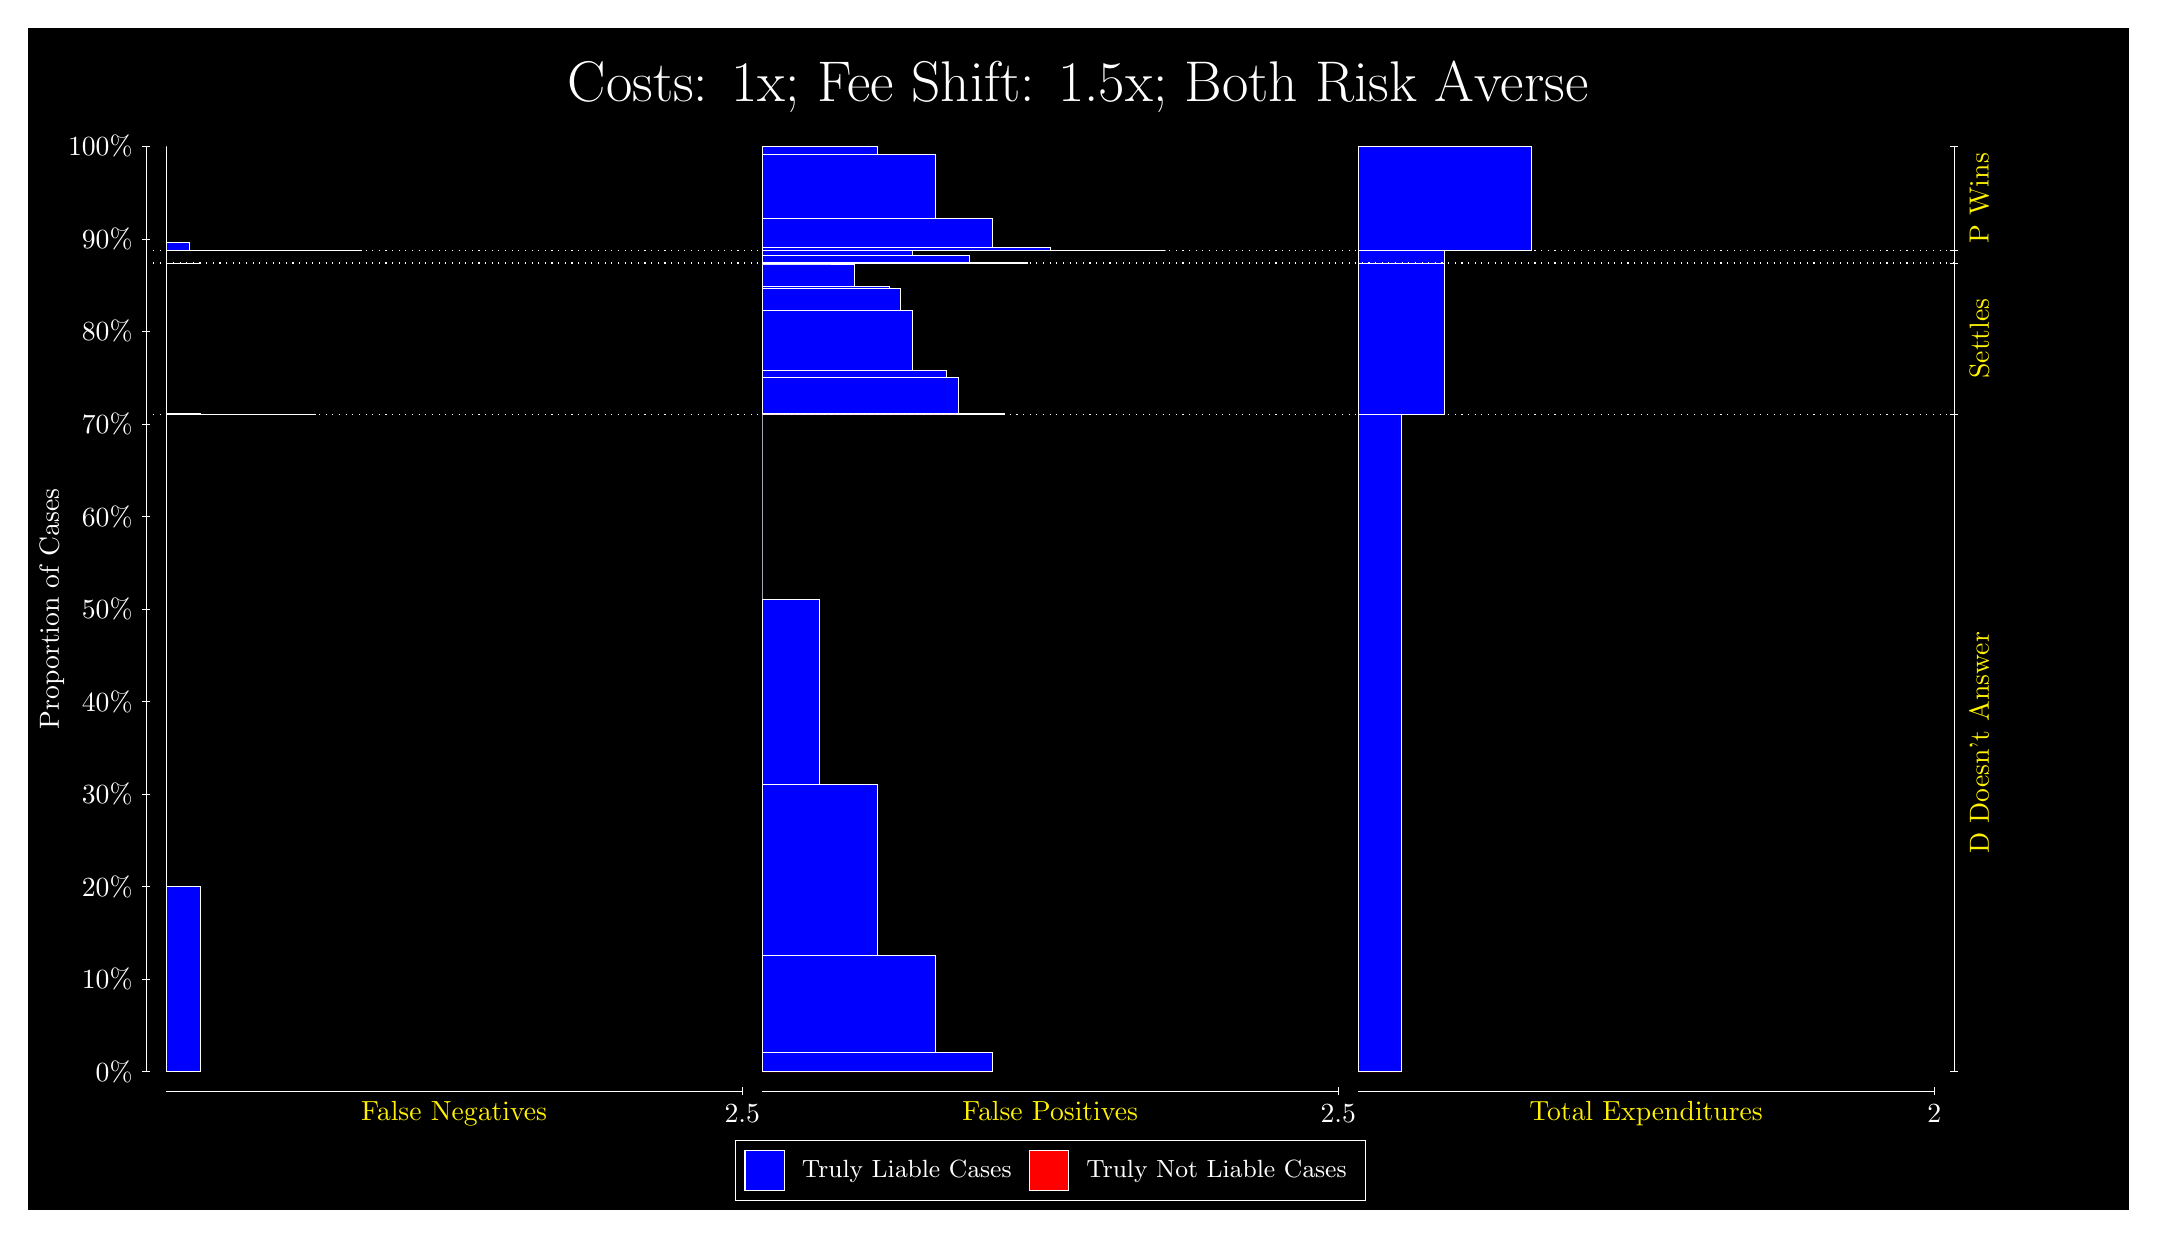
\begin{tikzpicture}
\draw[fill=black] (0,0) rectangle (26.667,15);
\draw[text=white] (0,13.5) rectangle (26.667,15) node[midway] {\huge Costs: 1x; Fee Shift: 1.5x; Both Risk Averse};
\draw[white, very thin] (1.5,1.75) -- (1.5,13.5);
\node[rotate=90, text=white, anchor=center] at (0.3, 7.625) {Proportion of Cases};
\draw[white, very thin] (1.45,1.75) -- (1.55,1.75);
\node[text=white, anchor=east] at (1.45, 1.75) {0\%};
\draw[white, very thin] (1.45,2.925) -- (1.55,2.925);
\node[text=white, anchor=east] at (1.45, 2.925) {10\%};
\draw[white, very thin] (1.45,4.1) -- (1.55,4.1);
\node[text=white, anchor=east] at (1.45, 4.1) {20\%};
\draw[white, very thin] (1.45,5.275) -- (1.55,5.275);
\node[text=white, anchor=east] at (1.45, 5.275) {30\%};
\draw[white, very thin] (1.45,6.45) -- (1.55,6.45);
\node[text=white, anchor=east] at (1.45, 6.45) {40\%};
\draw[white, very thin] (1.45,7.625) -- (1.55,7.625);
\node[text=white, anchor=east] at (1.45, 7.625) {50\%};
\draw[white, very thin] (1.45,8.8) -- (1.55,8.8);
\node[text=white, anchor=east] at (1.45, 8.8) {60\%};
\draw[white, very thin] (1.45,9.975) -- (1.55,9.975);
\node[text=white, anchor=east] at (1.45, 9.975) {70\%};
\draw[white, very thin] (1.45,11.15) -- (1.55,11.15);
\node[text=white, anchor=east] at (1.45, 11.15) {80\%};
\draw[white, very thin] (1.45,12.325) -- (1.55,12.325);
\node[text=white, anchor=east] at (1.45, 12.325) {90\%};
\draw[white, very thin] (1.45,13.5) -- (1.55,13.5);
\node[text=white, anchor=east] at (1.45, 13.5) {100\%};

\draw[white, very thin] (24.457,1.75) -- (24.457,13.5);
\draw[white, very thin] (24.407,1.75) -- (24.507,1.75);
\node[anchor=west] at (24.407, 1.75) {};
\draw[white, very thin] (24.407,10.099) -- (24.507,10.099);
\node[anchor=west] at (24.407, 10.099) {};
\draw[white, very thin] (24.407,12.018) -- (24.507,12.018);
\node[anchor=west] at (24.407, 12.018) {};
\draw[white, very thin] (24.407,12.181) -- (24.507,12.181);
\node[anchor=west] at (24.407, 12.181) {};
\draw[white, very thin] (24.407,13.5) -- (24.507,13.5);
\node[anchor=west] at (24.407, 13.5) {};

\draw[white, very thin, fill=blue] (1.75,1.75) rectangle (2.1891,4.0999);
\draw[white, very thin, fill=red] (1.75,4.0999) rectangle (1.75,4.0999);
\draw[white, very thin, fill=blue] (1.75,4.0999) rectangle (1.75,10.099);
\draw[white, very thin, fill=blue] (1.75,10.099) rectangle (3.6529,10.099);
\draw[white, very thin, fill=blue] (1.75,10.099) rectangle (3.0674,10.099);
\draw[white, very thin, fill=blue] (1.75,10.099) rectangle (2.921,10.099);
\draw[white, very thin, fill=blue] (1.75,10.099) rectangle (2.4819,10.099);
\draw[white, very thin, fill=blue] (1.75,10.099) rectangle (2.3355,10.099);
\draw[white, very thin, fill=blue] (1.75,10.099) rectangle (2.1891,10.108);
\draw[white, very thin, fill=red] (1.75,10.108) rectangle (1.75,10.108);
\draw[white, very thin, fill=blue] (1.75,10.108) rectangle (1.75,12.018);
\draw[white, very thin, fill=blue] (1.75,12.018) rectangle (2.1891,12.018);
\draw[white, very thin, fill=red] (1.75,12.018) rectangle (1.75,12.018);
\draw[white, very thin, fill=blue] (1.75,12.018) rectangle (1.75,12.181);
\draw[white, very thin, fill=blue] (1.75,12.181) rectangle (4.2384,12.181);
\draw[white, very thin, fill=blue] (1.75,12.181) rectangle (3.5065,12.181);
\draw[white, very thin, fill=blue] (1.75,12.181) rectangle (2.7746,12.181);
\draw[white, very thin, fill=blue] (1.75,12.181) rectangle (2.7746,12.182);
\draw[white, very thin, fill=blue] (1.75,12.182) rectangle (2.0428,12.183);
\draw[white, very thin, fill=blue] (1.75,12.183) rectangle (2.0428,12.287);
\draw[white, very thin, fill=red] (1.75,12.287) rectangle (1.75,12.287);
\draw[white, very thin, fill=blue] (1.75,12.287) rectangle (1.75,13.5);
\draw[white, very thin, fill=red] (9.3189,1.75) rectangle (12.246,1.75);
\draw[white, very thin, fill=blue] (9.3189,1.75) rectangle (12.246,1.9895);
\draw[white, very thin, fill=blue] (9.3189,1.9895) rectangle (11.515,3.2248);
\draw[white, very thin, fill=blue] (9.3189,3.2248) rectangle (10.783,5.4004);
\draw[white, very thin, fill=blue] (9.3189,5.4004) rectangle (10.051,7.7489);
\draw[white, very thin, fill=blue] (9.3189,7.7489) rectangle (9.3189,10.099);
\draw[white, very thin, fill=red] (9.3189,10.099) rectangle (12.393,10.099);
\draw[white, very thin, fill=blue] (9.3189,10.099) rectangle (12.393,10.104);
\draw[white, very thin, fill=red] (9.3189,10.104) rectangle (11.807,10.104);
\draw[white, very thin, fill=blue] (9.3189,10.104) rectangle (11.807,10.573);
\draw[white, very thin, fill=blue] (9.3189,10.573) rectangle (11.661,10.654);
\draw[white, very thin, fill=red] (9.3189,10.654) rectangle (11.222,10.654);
\draw[white, very thin, fill=blue] (9.3189,10.654) rectangle (11.222,11.414);
\draw[white, very thin, fill=blue] (9.3189,11.414) rectangle (11.075,11.698);
\draw[white, very thin, fill=blue] (9.3189,11.698) rectangle (10.929,11.721);
\draw[white, very thin, fill=blue] (9.3189,11.721) rectangle (10.49,12);
\draw[white, very thin, fill=blue] (9.3189,12) rectangle (10.344,12.009);
\draw[white, very thin, fill=blue] (9.3189,12.009) rectangle (10.197,12.009);
\draw[white, very thin, fill=blue] (9.3189,12.009) rectangle (9.758,12.018);
\draw[white, very thin, fill=blue] (9.3189,12.018) rectangle (9.6116,12.018);
\draw[white, very thin, fill=blue] (9.3189,12.018) rectangle (9.4652,12.018);
\draw[white, very thin, fill=blue] (9.3189,12.018) rectangle (9.3189,12.018);
\draw[white, very thin, fill=red] (9.3189,12.018) rectangle (12.686,12.018);
\draw[white, very thin, fill=blue] (9.3189,12.018) rectangle (12.686,12.022);
\draw[white, very thin, fill=blue] (9.3189,12.022) rectangle (11.954,12.12);
\draw[white, very thin, fill=blue] (9.3189,12.12) rectangle (11.222,12.18);
\draw[white, very thin, fill=blue] (9.3189,12.18) rectangle (10.49,12.181);
\draw[white, very thin, fill=blue] (9.3189,12.181) rectangle (9.758,12.181);
\draw[white, very thin, fill=red] (9.3189,12.181) rectangle (14.442,12.181);
\draw[white, very thin, fill=blue] (9.3189,12.181) rectangle (14.442,12.181);
\draw[white, very thin, fill=red] (9.3189,12.181) rectangle (13.71,12.181);
\draw[white, very thin, fill=blue] (9.3189,12.181) rectangle (13.71,12.181);
\draw[white, very thin, fill=red] (9.3189,12.181) rectangle (12.978,12.181);
\draw[white, very thin, fill=blue] (9.3189,12.181) rectangle (12.978,12.218);
\draw[white, very thin, fill=red] (9.3189,12.218) rectangle (12.246,12.218);
\draw[white, very thin, fill=blue] (9.3189,12.218) rectangle (12.246,12.59);
\draw[white, very thin, fill=red] (9.3189,12.59) rectangle (11.515,12.59);
\draw[white, very thin, fill=blue] (9.3189,12.59) rectangle (11.515,13.394);
\draw[white, very thin, fill=blue] (9.3189,13.394) rectangle (10.783,13.498);
\draw[white, very thin, fill=blue] (9.3189,13.498) rectangle (10.051,13.5);
\draw[white, very thin, fill=blue] (9.3189,13.5) rectangle (9.3189,13.5);
\draw[white, very thin, fill=red] (16.888,1.75) rectangle (17.437,1.75);
\draw[white, very thin, fill=blue] (16.888,1.75) rectangle (17.437,10.099);
\draw[white, very thin, fill=red] (16.888,10.099) rectangle (17.986,10.099);
\draw[white, very thin, fill=blue] (16.888,10.099) rectangle (17.986,12.018);
\draw[white, very thin, fill=red] (16.888,12.018) rectangle (17.986,12.018);
\draw[white, very thin, fill=blue] (16.888,12.018) rectangle (17.986,12.181);
\draw[white, very thin, fill=red] (16.888,12.181) rectangle (19.083,12.181);
\draw[white, very thin, fill=blue] (16.888,12.181) rectangle (19.083,13.5);
\draw[white, dotted] (1.5,10.099) -- (24.457,10.099);
\draw[white, dotted] (1.5,12.018) -- (24.457,12.018);
\draw[white, dotted] (1.5,12.181) -- (24.457,12.181);
\draw[white, very thin] (1.75,1.5) -- (9.0689,1.5);
\node[text=yellow, anchor=north] at (5.4094, 1.5) {False Negatives};
\draw[white, very thin] (9.0689,1.45) -- (9.0689,1.55);
\node[text=white, anchor=north] at (9.0689, 1.45) {2.5};

\draw[white, very thin] (9.3189,1.5) -- (16.638,1.5);
\node[text=yellow, anchor=north] at (12.978, 1.5) {False Positives};
\draw[white, very thin] (16.638,1.45) -- (16.638,1.55);
\node[text=white, anchor=north] at (16.638, 1.45) {2.5};

\draw[white, very thin] (16.888,1.5) -- (24.207,1.5);
\node[text=yellow, anchor=north] at (20.547, 1.5) {Total Expenditures};
\draw[white, very thin] (24.207,1.45) -- (24.207,1.55);
\node[text=white, anchor=north] at (24.207, 1.45) {2};

\node[text=yellow, centered, rotate=90] at (24.777, 5.9244) {D Doesn't Answer};
\node[text=yellow, centered, rotate=90] at (24.777, 11.058) {Settles};

\node[text=yellow, centered, rotate=90] at (24.777, 12.84) {P Wins};

\draw (12.978300999999998,1.5) node[draw=none] (baseCoordinate) {};
\begin{scope}[align=center]
        \matrix[scale=0.5, draw=white, below=0.5cm of baseCoordinate, nodes={draw}, column sep=0.1cm]{
            \node[rectangle, draw, minimum width=0.5cm, minimum height=0.5cm, fill=blue] {}; &
            \node[draw=none, font=\small, text=white] (B) {Truly Liable Cases}; &
            \node[rectangle, draw, minimum width=0.5cm, minimum height=0.5cm, fill=red] {}; &
            \node[draw=none, font=\small, text=white] (B) {Truly Not Liable Cases}; \\
            };
\end{scope}

\end{tikzpicture}
\end{document}